\documentclass[11pt]{article}
\usepackage[spanish]{babel}
\usepackage[utf8]{inputenc}
\usepackage[T1]{fontenc}
\usepackage{graphicx}
\topmargin=-1.2cm
\textheight=22cm
\textwidth=16cm  
\oddsidemargin=0.45cm  
\setlength{\parindent}{0cm}
\renewcommand{\baselinestretch}{1.1}
\graphicspath{{hola/}}
\title{Evaluación 2}
\author{Hinostroza Moya Natalia}
\date{26 de abril de 2017}

\begin{document}
%===============================================================================
% PORTADA
%===============================================================================
\begin{titlepage}
\begin{center}
\includegraphics[scale=0.35]{escudo.png}
\end{center}
\vspace*{0.02in}
\begin{center}

\rmfamily\textbf{\LARGE UNIVERSIDAD DE SONORA}\\
\vspace*{1.02in}
{\Large División de Ciencias Exactas y Naturales}\\
{\Large Departamento de Física}\\

\vspace*{0.99in}
\rule{99mm}{0.1mm}\\
\vspace*{0.4cm}
\textbf{\LARGE Evaluación 2}\\
\vspace*{0.001in}
\rule{99mm}{0.1mm}

\vspace*{1in}
\normalsize{Autor:}\
\normalsize{Natalia Hinostroza Moya}\\
\vspace*{0.3mm}
\normalsize Profesor:\
\normalsize Carlos Lizárraga Celaya\\
\vspace*{1.5cm}
\normalsize 26 de abril de 2017

\end{center}
\end{titlepage}
%==============================================================================
% DESARROLLO
%==============================================================================
\textbf{\section*{\LARGE Resumen}}
En este reporte se hace una síntesis de lo que se llevo a cabo para realizar la segunda evaluación de la clase de Computacional. Así mismo vienen los cuestionamientos que se te piden respondas con lo obtenido en la actividad realizada para la evaluación. 

En la evaluación se pedía lo siguiente:\\

\begin{enumerate}
\item \textbf{De los datos proporcionados, utiliza una transformada discreta de Fourier, para encontrar la frecuencia del ciclo principal. Muestra una gráfica con los principales modos encontrados.}\\

A continuación se muestra el comando con el que se aplicó la transformada de Fouriel junto a a gráfica obtenida con la frecuencia principal indicada. 

\begin{verbatim}
#Aplicar la transformada de Fourier
N= 3213
T = 1.0

#Tamaño de la imagen
fig = plt.gcf()
fig.set_size_inches(13, 8)

y = df["Manchas"] 
yf = fft(y)
xf = fftfreq(N, T)
xf = fftshift(xf)
yplot = fftshift(yf)

graf = plt.plot(xf, 2.0/N *abs(yplot))
plt.xlim(0,0.02)
plt.ylim(0,50)
plt.grid(True)

plt.xlabel('Frecuencia')
plt.ylabel('Número de Manchas')
plt.title('Manchas Solares')
plt.text(0.007,41,'11.11 años')

fig = plt.gcf()
fig.set_size_inches(14, 7)
plt.show()
\end{verbatim}

\begin{center}
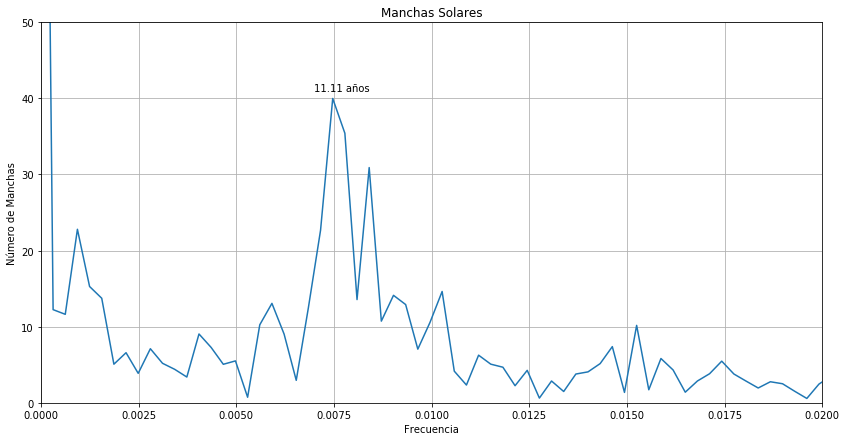
\includegraphics[scale=0.50]{grafi.png}
\end{center}

\vspace{1cm}

\item\textbf{¿Encuentras un solo ciclo principal o un conjunto de ciclos con frecuencia cercana? ¿Cuál sería el promedio del conjunto de frecuencias?}\\

Tercer armónico\\
Amplitud= 11.3390760528\\
frecuencia= 0.00715841892312\\
periodo= 11.73\\

Cuarto armónico\\
Amplitud= 19.9936166043\\
frecuencia= 0.00746965452848\\
periodo= 11.11\\

Quinto armónico\\
Amplitud= 17.7099160016\\
frecuencia= 0.00778089013383\\
periodo= 10.68\\

promedio de periodo= 11.17

\item\textbf{¿Que otros ciclos relevantes encuentras? Proporciona una tabla con las amplitudes de los ciclos.}


\begin{table}[htbp]
\begin{center}
\begin{tabular}{|l|l|l|}
\hline \hline
Amplitud & Frecuencia & Periodo  \\
\hline \hline
11.3390760528 & 0.00715841892312 & 11.73 años \\ \hline
19.9936166043
 & 0.00746965452848 & 11.26 años \\ \hline
17.7099160016 & 0.00778089013383 & 10.68años \\ \hline
15.4540189405 & 0.00840336134454
 & 9.92 años \\ \hline

\end{tabular}
\label{tabla:sencilla}
\end{center}
\end{table}

\item\textbf{Lo que han encontrado hasta ahora son ciertas regularidades, incluso hay pronósticos de un rango para el número de manchas solares. ¿Cómo crees que es posible predecir el número de manchas?}

Analizando cómo va variando la aparición de manchas con respecto al tiempo. Y con ello crear una función que nos ayude a predecir la apricion de las manchas. 

\end{enumerate}
\end{document} 

